\section{Effects of TR}\label{sec:load}
\subsection{Effect on Load}
The dipping and peaking of the magnitude of the frequency response plot of a system with TR is not the
only effect that TR has on the system. Another effect is a change in the effective load seen by the system
before $\omega_{ar}$ to after $\omega_r$, see Fig.~\ref{fig:trBode}. Before the $\omega_{ar}$ the acting inertial load on the system is the sum of the
actuator�s inertial load, $J_a$, and the load�s inertial load, $J_L$. This is a second order system with a slope of
negative $40\frac{dB}{dec}$ on the frequency response plot. After the $\omega_{r}$ the acting inertial load is only the
actuator�s inertia, $J_a$, which also defines a second order system with a slope of negative $40\frac{dB}{dec}$ on the
frequency response plot. The latter characteristics can be seen in the frequency response plot in Fig.~\ref{fig:trBode}.

\noindent Transfer function for a mass spring damper system with effective load of $J_a+J_L$, ideal coupler (pre-$\omega_{ar}$)

\begin{equation}
\frac{\theta_{J_a+J_L}(s)}{T(s)=\frac{1}{(J_a+J_L)s^2}}
\end{equation}

\noindent Transfer function for a mass spring damper system with effective load of $J_a$, ideal coupler (post-$\omega_{r}$)
\begin{equation}
\frac{\theta_{J_a(s)}}{T(s)=\frac{1}{J_as^2}}
\end{equation}


It can be noted that there is an offset between the frequency responses of the second order estimations of
the system with TR when going from before the war to after the $\omega_{r}$ when looking at the magnitude in $dB$ of
the response. This offset, known as gain separation, means that there is a parameter, in this case the
effective inertia on the system, which is changing. Fig.~\ref{fig:trBode} shows the frequency response of the system
with TR from Eq.~\ref{eq:tf} and values from Table~\ref{table:defaultVals} with the added frequency responses of a systems with out
TR but having the effective load as $J_L+J_a$ and $J_a$.  This is referred to as load switching.

\begin{center}
	\begin{table}
	\caption{Values used for TR model based on the PITTMAN\textsuperscript{\texttrademark} N2314 series brushless DC servo motor and a custom inertial load/coupler}
	\begin{center}
  \begin{tabular}{ c | c | c | c }

    					& Inertia 'J' 								&	Damping 'B' 												&	Spring 'K'  									\\ 
    					& ($oz-in-sec^2$)							&	($\frac{oz-in}{krpm}$)							&	$\frac{oz}{in}$) 							\\ \hline
    Actuator 	& 0.0023 											& 0																		& 0															\\ \hline
    Coupler 	& 0 													& 0.005 															& 55														\\ \hline
    Load 			& 0.0033 											& 0																		& 0															\\

  \end{tabular}
  \end{center}
  \label{table:defaultVals}
  \end{table}
\end{center}





\subsection{Effect on Velocity}

When there is a step torque command input to the system, like that seen in Fig.~\ref{fig:torqueIn} (top), the output velocity
exhibits an oscillatory behavior. The frequency of oscillation is expected to be equal to $\omega_r$ of the system
from Eq.~\ref{eq:tf}. Therefore this should have a ripple frequency of 201.4 rad/sec, 32.1 Hz.

\begin{figure}[ht]
  \centering
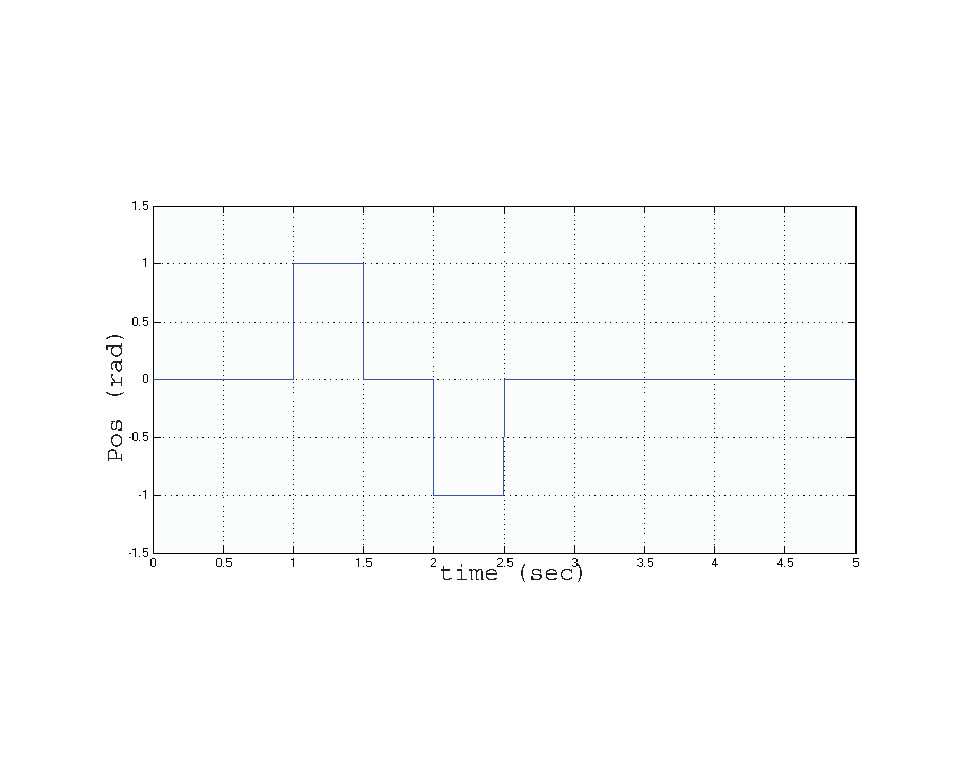
\includegraphics[width=0.8\columnwidth]{./pix/posIn2.pdf}\\
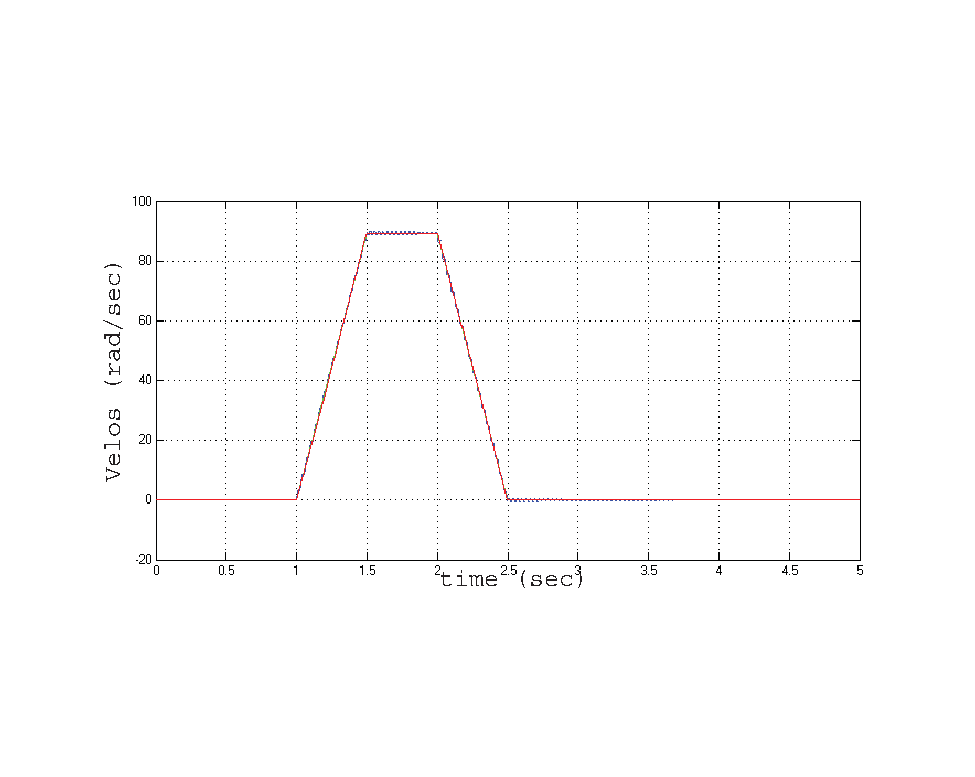
\includegraphics[width=0.8\columnwidth]{./pix/velosOut2.pdf}
  \caption{(TOP) Step Torque Input to TR System. Vertical Axis is Magnitude, Horizontal
Axis is Time in sec.  (BOTTOM) Angular Velocity of the Actuator Shaft of the system with TR (Yellow), Angular Velocity
of the Actuator Shaft of the system without TR (Pink) due to the torque input. Vertical Axis is
Magnitude, Horizontal Axis is Time in sec.}
  \label{fig:torqueIn}
\end{figure}


\begin{figure}[ht]
  \centering
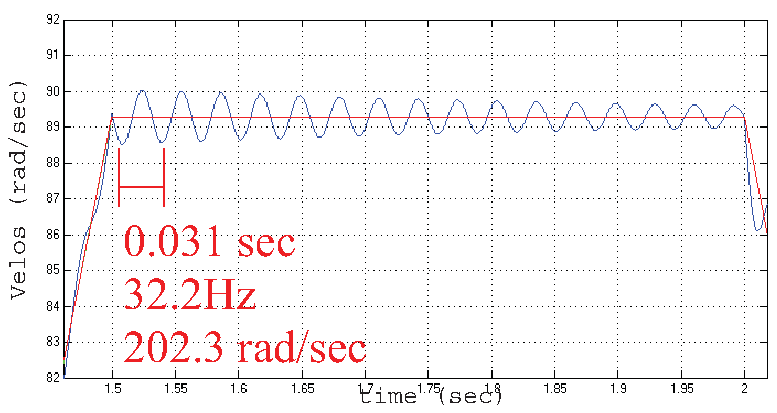
\includegraphics[width=1.0\columnwidth]{./pix/velosOutClose2.pdf}
  \caption{Angular velocity of the actuator shaft $\dot{\theta}_a$ for the system with TR (Blue), Angular Velocity of
the actuator shaft for the system without TR (Red) due to the torque input zoomed in from 1.5 to
2.0 sec. Vertical Axis is Magnitude, Horizontal Axis is Time in sec}
  \label{fig:trap}
\end{figure}


Figure 16 shows Fig.\ref{fig:trap} magnified about 1.5 sec to 2 sec. The angular velocity of
the actuator shaft has a decaying sinusoid on it due to the resonance and the spring/damping.  
The period of is 0.031sec (32.2 Hz, 202.3 rad/sec). This frequency is the
same as the $\omega_r$ computed in Eq.\ref{eq:tf}, shown in Fig.~\ref{fig:trBode} and uses the values in Table~\ref{table:defaultVals}.  
This frequency $\omega_n$ can by calculated by

\begin{equation}
\omega_n=\sqrt{\frac{K_c(J_a+J_L)}{J_aJ_L}}
\end{equation}





